\section{Морфологическая обработка данных и анализ текста}

В данной секции в качестве входа используются файлы, полученные после запуска экстрактора, описанного в предыдущений секции. В целях сохранения независимости этапов обработки, а также избежание повторного запуска экстрактора была написана отдельная утилита \href{https://github.com/vasalf/hse-web-search-homework/blob/master/1/apply.py}{apply.py}, осуществляющая обработку текста, очищенного от html-тэгов и подсчёт статистик. 

\paragraph{Архитектура}

Для более эффективного использования ресурсов, гибкости разработки и минимализации конфликтов между разработчиками был реализован \href{https://refactoring.guru/ru/design-patterns/chain-of-responsibility}{паттерн проектирования pipeline}. Утилита послеовательно принимает на вход файлы и пропускает их через пайплайн, состоящий из необходимого нам набора обработчиков, которые, благодаря шаблону, могут разрабатываться независимо, просто наследуясь от интерфейса обработчика. Набор и последовательность обработчиков при необходимости можно легко изменить в зависимости от наших потребностей.

Для решения текущей задачи был реализован следующий набор обработчиков (в порядке запуска):

\begin{enumerate}
	\item TextProcessorStage -- преобразует текст в набор лемматизированных слов
	\item JsonUnpackerStage -- распаковывает JSON в текстовом представлении в настоящий JSON
	\item GraphBuilder -- собирает метаданные о ссылочных рёбрах из JSONа, распакованного предыдущим обработчиком
	\item StopwordsCounter -- подсчитывает слова из лемматизированного текста, классифицируемые как стоп-слова 
	\item DictionaryStats -- собирает словари слов, ведёт на их основе подсчёт tf-idf
	\item SimpleStats -- собирает простую статистику, не требующую хранения данных или использования внешних библиотек (например, среднюю длину слов).	
\end{enumerate}

После того, как какждый документ был обработан пайплайном, у каждого обработчика вызывается метод dump, обрабатывающий полученные результаты, после чего происодит вывод на экран/запись результатов в файл/рендеринг графика и т.д. 

В случае необходимости такую архитектуру можно легко распараллелить по данным, создав несколько экземпляров пайплайна и распределив между ними файлы. 

Для большей наглядности ниже приведена диграмма классов: 

\begin{figure}
	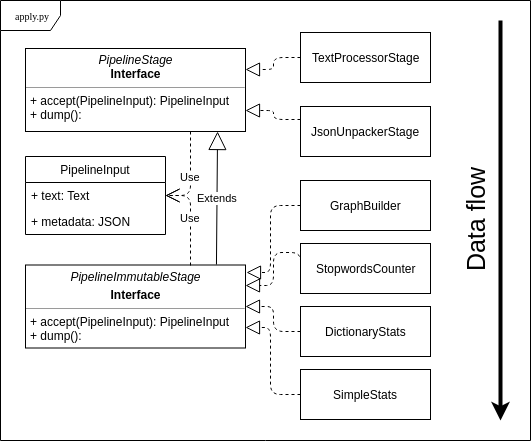
\includegraphics[width=.5\textwidth]{apply_uml_data_flow.png}
	\caption{UML-диаграмма классов пайплайна}
	\label{apply-uml}
\end{figure}

Классы, унаследованные от \texttt{PipelineImmutableStage} гаранитированно пропустят через себя \texttt{PipelineInput} без изменений. Это сделано, чтобы дополнительно обезопасить себя от ошибок.


\paragraph{Обработка текста}

Полученный от экстрактора файл конкатенировался в одну строку, переводился в нижний регистр, после чего токенизировался и леммматизировался с помощью библиотеки \texttt{mystem} методом \texttt{Mystem.lemmatize}. После этого полученный набор токенов фильтровался на предмет принадлежности множеству слов на одном из трёх языков: русском, беларусском или английском. 

Токен считается:
\begin{itemize}
	\item Словом на английском языке, если он состоит исключительно из букв набора ''abcdefghijklmnopqrstuvwxyzéôïç'' (некоторые слова английского языка имеют французское происхождение).
	
	\item Словом на русском языке, если он состоит исключительно из букв набора ''абвгдеёжзийклмнопрстуфхцчшщьыъэюя''
	
	\item Словом на английском языке, если он состоит исключительно из букв набора ''абвгдеёжзiйклмнопрстуўфхцчшьыэюя''
\end{itemize}

Сразу стоит оговориться, что для некоторых слов мы не можем сказать, на русском или беларусском языке оно написано ввиду большого пересечения алфавитов, поэтому многие из последующих статистик посчитаны для русских и балорусских слов вместе.

Также стоит заметить, что и белорусский, и русский алфавиты содержат в себе буквы, которые отсутствуют в другом языке (например, в русском нет буквы 'ў', а в белорусском 'и'), поэтому слова, состоящие из букв объединения алфавитов, но не принадлежащие ни одному алфавиту по отдельности, были отфильтрованы такой проверкой, хотя и могли иметь смысл . Тем не менее, таких слов пренебрежимо мало и их можно опустить.


\paragraph{Подсчёт статистик}

